\documentclass[a4paper,12pt]{article}
\usepackage[latin1]{inputenc}
%\usepackage[spanish]{babel}
\usepackage{amssymb}
\usepackage{graphicx}
%\usepackage{textcomp}
\usepackage{geometry}
\geometry{margin=1in}
\usepackage{cite}
\usepackage{url}
\usepackage{hyperref}
\usepackage{float}
\usepackage{amsmath}
\usepackage{cleveref}

\crefformat{footnote}{#2\footnotemark[#1]#3}

\title{\textbf{Project 2: Classical Planning}}
\author{Miguel Tasende}

%opening
\begin{document}


\maketitle

\section{Introduction}


\section{Problems 1 and 2}
The first two problems were solved using each of the search algorithms. The results can be seen on the table below.

\begin{figure}[!h]
\centering
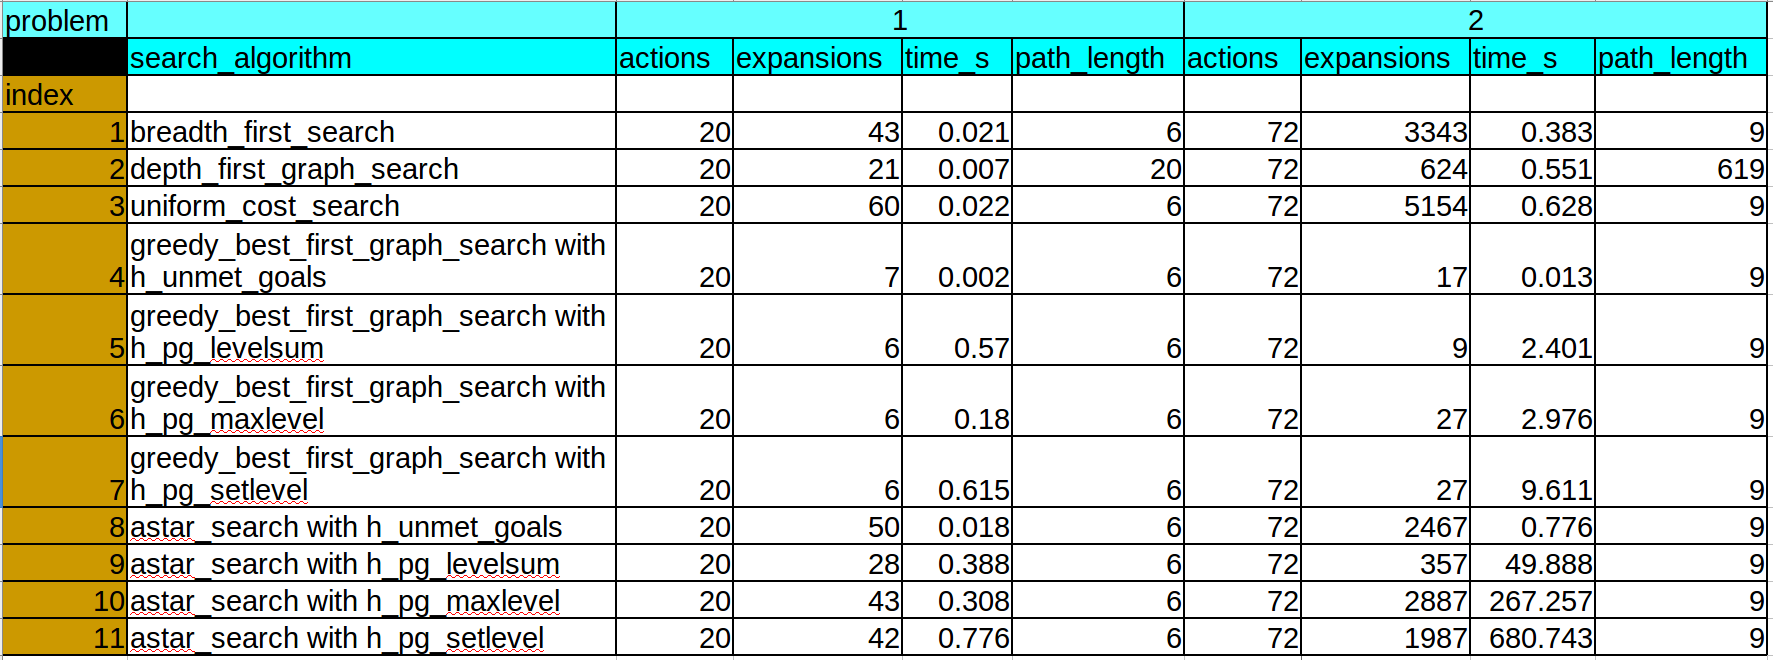
\includegraphics[width=6.0in]{results/results12.png}
\caption{Results for the first two problems, with all the search algorithms}
\label{fig_raw_data}
\end{figure}

It was noticed that the Depth First algorithm was resulting in extremely long paths, and considering this is an Air Cargo problem, it is reasonable to expect that optimum or near-optimum solutions are searched for. Therefore, the Depth First algorithm won't be considered in the rest of the project.\\
$A^*$ with ``maxlevel'' and ``setlevel'' heuristics are taking a lot of time to find a solution, but they will be considered for the other problems, to have more data (it is expected that running all the remaining combinations may take about 10 hours of processing with pypy3).

\section{Problems 3 and 4}
Problems 3 and 4 were solved with all the algorithms except Depth First. The results are below.


\section{Aggregated Results}
Some tables and charts are shown below, aggregating the results for all problems, and all search algorithms in different ways.

\section{Results Analysis}
\subsection{Which algorithm or algorithms would be most appropriate for planning in a very restricted domain (i.e., one that has only a few actions) and needs to operate in real time?}


\subsection{Which algorithm or algorithms would be most appropriate for planning in very large domains (e.g., planning delivery routes for all UPS drivers in the U.S. on a given day)}


\subsection{Which algorithm or algorithms would be most appropriate for planning problems where it is important to find only optimal plans? }



\begin{figure}[!h]
\centering
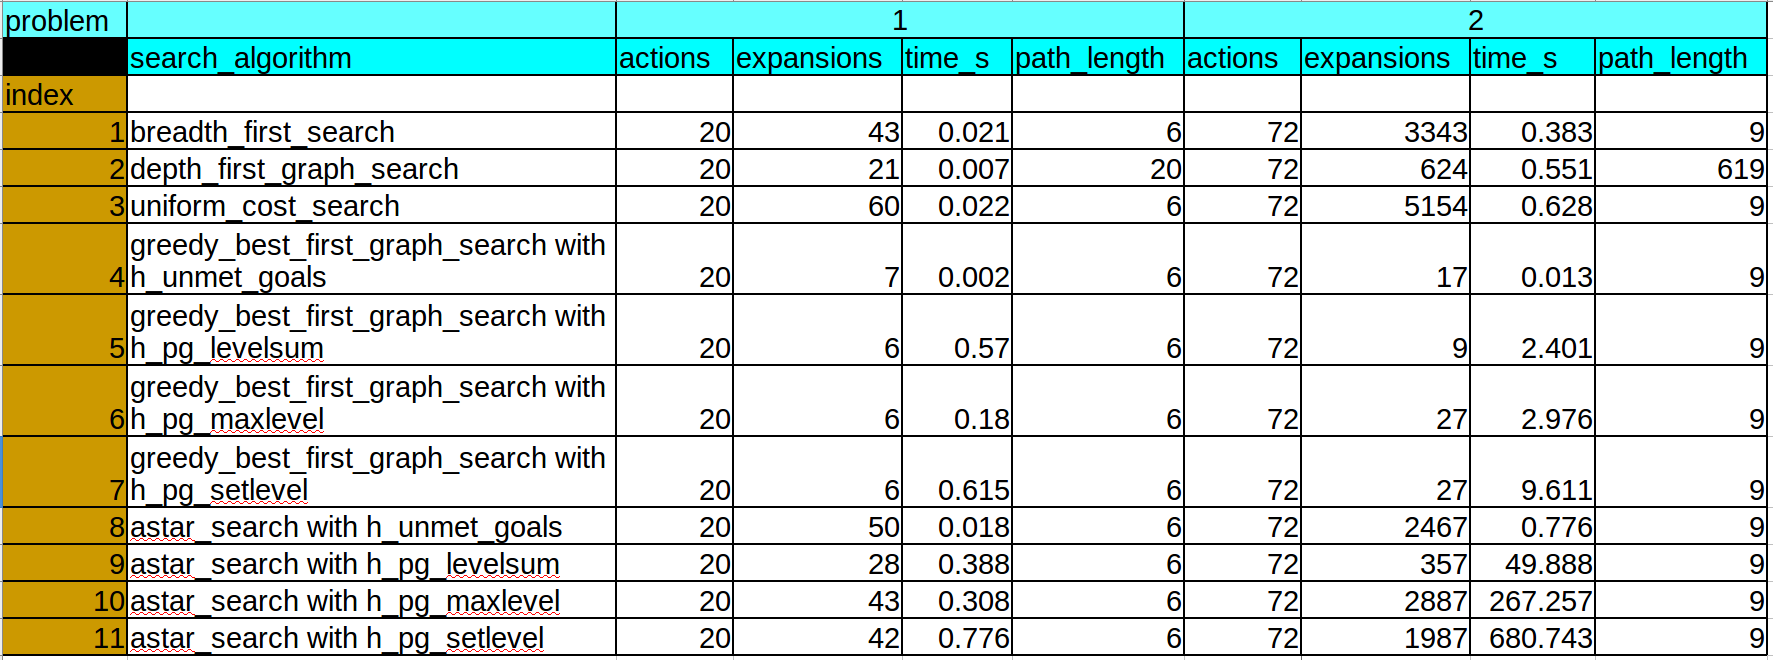
\includegraphics[width=5.0in]{results/results12.png}
\caption{CAPTION HERE!}
\label{fig_raw_data}
\end{figure}

\end{document}